\documentclass[12pt]{article}
\usepackage{float}
\usepackage{svg} 
\usepackage{sbc-template}
\usepackage{amsmath}
\usepackage{graphicx,url}
\usepackage{indentfirst}
\usepackage{amsfonts} 
%\usepackage[brazil]{babel}   
\usepackage[utf8]{inputenc}  
\usepackage{svg}
\usepackage{multirow}
\usepackage{multicol}
\usepackage[brazil]{babel}   
\usepackage[utf8]{inputenc} 
\usepackage{rotating}
\usepackage{geometry}
\geometry{a4paper, margin=1in}
\usepackage{array}
\usepackage[table]{xcolor}
\definecolor{goldrank}{RGB}{184,142,0}
\definecolor{silverrank}{RGB}{100,100,100}
\definecolor{bronzerank}{RGB}{150,90,30} 
\definecolor{third}{RGB}{102, 51, 153} %light purple
\definecolor{second}{RGB}{230, 126, 34} % orange
\definecolor{first}{RGB}{22, 160, 134} % blue
\sloppy

\title{ST-MTLNet: Representações Espaço-Temporais \\de Pontos de Interesse para Aprendizado Multitarefa}


\author{ Tarik S. Paiva\inst{1}, Vitor H. O. Silva\inst{1}, Germano B. dos Santos\inst{1}, Fabrício A. Silva\inst{1}}

\address{Laboratório de Inteligência em Sistemas Pervasivos e Distribuídos (NESPeD-LAB)\\ Universidade Federal de Viçosa, Florestal, MG, Brasil
 \email{\{tarik.paiva, vitor.oliveira, germano.santos, fabricio.asilva\}@ufv.br}
}

\begin{document} 

\maketitle

\begin{abstract}
This work proposes ST-MTLNet, a multi-task architecture for POI Category Classification and Next-POI Prediction based on decoupled representations. The model combines a continuous spatial encoder for geographic coordinates, a temporal encoder (Time2Vec) for visitation patterns, and a hierarchical categorical encoder (HGI) for structural and regional POI context. Two spatial encoders, SIREN and Sphere2Vec-M, originally proposed for remote sensing and ecology tasks, are evaluated in the context of multi-task POI modeling on LBSNs. Experiments on the Gowalla dataset across Florida, California, and Texas show that the proposed approach outperforms the baseline in all 21 category-state combinations for classification, with average gains of 20--24 percentage points, and in 76\% of combinations for next-POI prediction. The comparison between spatial encoders also reveals complementary performance profiles associated with the geographic distribution of POIs in each territory.
\end{abstract}

\begin{resumo}
Este trabalho propõe o ST-MTLNet, uma arquitetura multitarefa para classificação de categoria de POI e predição do próximo POI baseada em representações desacopladas. O modelo combina uma representação espacial contínua para coordenadas geográficas, uma representação temporal (Time2Vec) para padrões de visitação e uma representação categórica hierárquica (HGI) para contexto estrutural e regional dos POIs. Duas arquiteturas de codificação espacial, SIREN e Sphere2Vec-M, originalmente propostas para sensoriamento remoto e ecologia, são avaliadas no contexto de tarefas multitarefa de POIs em LBSNs. Experimentos com o dataset Gowalla nos estados da Flórida, Califórnia e Texas demonstram que a abordagem proposta supera o \textit{baseline} em todas as 21 combinações de categoria e estado para classificação, com ganhos médios de 20 a 24 pontos percentuais, e em 76\% das combinações para predição do próximo POI. A comparação entre as arquiteturas espaciais revela ainda perfis complementares de desempenho associados à distribuição geográfica dos POIs em cada território.
\end{resumo}


\section{Introdução}
Redes Sociais Baseadas em Localização (\textit{Location-Based Social Networks}, LBSNs), como o Gowalla \cite{cho2011friendship,jure2014snap}, registram \textit{check-ins} de usuários com localização geográfica, horário de visita e categoria do local visitado. Nesse contexto, um Ponto de Interesse (POI) corresponde a um local físico semanticamente identificável, como restaurantes, lojas, aeroportos ou parques. A análise desses dados é relevante para aplicações como recomendação e mobilidade urbana. Nesse cenário, duas tarefas se destacam:

\begin{enumerate}
    \item \textbf{Classificação de Categoria de POI}: classificar a categoria semântica (e.g., \textit{Food}, \textit{Shopping}, \textit{Travel}) de um POI a partir de suas características.
    \item \textbf{Predição do Próximo POI}: prever a categoria do próximo POI que um usuário visitará, dada a sequência histórica de seus \textit{check-ins}.
\end{enumerate}

Em princípio, essas tarefas podem ser tratadas como relacionadas, pois compartilham a mesma base de dados de mobilidade e o mesmo espaço semântico de categorias, o que torna o aprendizado multitarefa (\textit{Multitask Learning}, MTL) uma estratégia promissora para explorar informação compartilhada entre elas \cite{caruana1997multitask}. No entanto, elas impõem demandas distintas. A classificação de categoria de POI é uma tarefa não sequencial, pois depende principalmente dos atributos do próprio POI e de seu contexto espacial. Já a predição do próximo POI é explicitamente sequencial, exigindo a modelagem de ordem temporal, recorrência e transições ao longo da trajetória do usuário. Assim, as informações úteis para uma tarefa podem não beneficiar a outra da mesma forma.

O MTLNet, proposto em \cite{silva2025mtlnet}, explora esse potencial ao modelar as duas tarefas em uma única arquitetura multitarefa com compartilhamento rígido de parâmetros. No entanto, o modelo utiliza exclusivamente representações vetoriais baseadas na estrutura do grafo, geradas pelo\textit{ Deep Graph Infomax} (DGI), que codifica informações espaciais e categóricas em um único vetor de 64 dimensões, sem incorporar explicitamente coordenadas geográficas contínuas nem padrões temporais de visitação.

Diante disso, surge o questionamento se a decomposição da entrada em \textit{encoders} especializados para espaço, tempo e categoria produz uma base mais adequada para as duas tarefas do que o \textit{embedding} monolítico do DGI. A hipótese é que representações desacopladas capturam dimensões complementares da mobilidade humana que não são modeladas explicitamente pela abordagem original.

Nesse sentido, este trabalho propõe o ST-MTLNet (\textit{Spatial-Temporal MTLNet}), que integra três representações independentes: uma representação espacial contínua para coordenadas geográficas, uma representação temporal (Time2Vec) para padrões de visitação e uma representação categórica hierárquica para relações regionais e estruturais entre POIs. Na dimensão espacial, avaliamos duas arquiteturas com pressupostos distintos, SIREN e Sphere2Vec-M, originalmente validadas em tarefas geoespaciais de sensoriamento remoto e ecologia \cite{wu2024torchspatial}, mas ainda pouco exploradas no aprendizado multitarefa de POIs em LBSNs.

Os experimentos foram realizados com a base pública Gowalla \cite{jure2014snap} nos estados da Flórida, Califórnia e Texas. Na classificação categórica, o ST-MTLNet supera o MTLNet em todas as combinações de categoria e estado avaliadas, com ganhos médios de 20 a 24 pontos percentuais. Na predição do próximo POI, o modelo proposto vence na maioria dos cenários, com destaque para categorias como \textit{Food}. A comparação entre SIREN e Sphere2Vec-M mostra ainda que, embora a abordagem modular seja consistentemente superior ao \textit{baseline}, o \textit{encoder} espacial mais adequado depende da distribuição geográfica dos POIs em cada território.

Portanto, as principais contribuições deste trabalho são:
\begin{itemize}
\item A proposição do ST-MTLNet, que incorpora representações espaciais contínuas, temporais e categóricas hierárquicas ao MTLNet.

\item A avaliação comparativa de SIREN e Sphere2Vec-M em três estados com estruturas territoriais distintas.

\item A disponibilização pública do código-fonte e do \textit{pipeline} experimental.\footnote{O código-fonte completo está disponível em \url{https://github.com/TarikSalles/Spatial_Embeddings}}
\end{itemize}

A organização deste trabalho segue o seguinte formato: a Seção \ref{sec:related_works} apresenta os trabalhos relacionados. A Seção \ref{sec:methods} descreve a metodologia proposta. A Seção \ref{sec:results} discute os resultados experimentais. Por fim, a Seção \ref{sec:conclusion} apresenta as conclusões e trabalhos futuros.


\section{Trabalhos Relacionados} \label{sec:related_works}
A predição e classificação de POIs são desafios fundamentais em sistemas de recomendação baseados em localização e em análise de mobilidade urbana. Esta seção organiza os trabalhos relacionados em quatro eixos: representações baseadas em grafos, codificadores espaciais, representações temporais e aprendizado multitarefa aplicado a POIs.

\subsection{Representações de POIs Baseadas em Grafos}

A modelagem de POIs por meio de grafos permite capturar relações de vizinhança espacial e semântica entre locais. O modelo POI2Vec \cite{feng2017poi2vec} adapta a arquitetura Word2Vec para gerar \textit{embeddings} de POIs que incorporam a influência geográfica entre locais por meio de uma estrutura de árvore binária geográfica. O CATAPE (\textit{Category-Aware Location Embedding}) \cite{rahmani2019category} estende essa ideia incorporando informações categóricas e sequenciais, capturando a influência geográfica entre POIs com base na sequência temporal de visitas dos usuários.

Em uma abordagem auto-supervisionada, o \textit{Deep Graph Infomax} (DGI) \cite{velickovic2019deep} maximiza a informação mútua entre representações locais (nós) e globais (grafo) para gerar \textit{embeddings} sem supervisão explícita. O HGI (\textit{Hierarchical Graph Infomax}) \cite{huang2023learning} avança sobre essa linha ao operar em múltiplos níveis hierárquicos (POI, região e cidade), produzindo representações enriquecidas com informações regionais por meio de convoluções em grafos e mecanismos de multi-atenção. 
% O HAVANA \cite{dos2024havana} combina \textit{Graph Attention Networks} (GAT) \cite{velivckovic2017graph} com filtros ARMA para anotação semântica de locais, mostrando a eficácia de modelos híbridos de grafos para a tarefa de classificação categórica.

No entanto, essas abordagens codificam informações espaciais de forma implícita por meio da topologia do grafo, sem utilizar diretamente as coordenadas geográficas como sinal de entrada para a representação.

\subsection{Representações Espaciais}

O uso direto de coordenadas geográficas para a geração de características latentes espaciais é uma abordagem distinta das representações baseadas em grafos. O \textit{framework} TorchSpatial \cite{wu2024torchspatial} estabelece um \textit{benchmark} unificado para a avaliação de estratégias de representação espacial, permitindo a comparação sistemática entre diferentes arquiteturas.

% O Space2Vec \cite{mai2020multiscalerepresentationlearningspatial} propõe uma codificação posicional multi-escala inspirada em \textit{grid cells} do sistema nervoso, utilizando funções senoidais com frequências logaritmicamente espaçadas para transformar coordenadas em representações vetoriais. A abordagem 
A metodologia SIREN (\textit{Sinusoidal Representation Networks}) \cite{sitzmann2020implicit}, aplicada ao contexto geográfico \cite{rußwurm2024geographiclocationencodingspherical}, modela funções contínuas por meio de ativações senoidais, sendo capaz de representar sinais de alta frequência em dados espaciais. O Sphere2Vec \cite{mai2023sphere2vecgeneralpurposelocationrepresentation} opera diretamente sobre coordenadas esféricas com múltiplas escalas de resolução, preservando propriedades de distância geodésica que são perdidas em projeções planares.

Embora essas estratégias tenham sido avaliadas em tarefas geoespaciais como predição de espécies e estimativa de população, sua aplicação pode ser estendida para modelos de predição e classificação de POIs como proposto neste trabalho.

\subsection{Representações Temporais}

A dimensão temporal é central para tarefas de predição de POIs, uma vez que os padrões de visitação dos usuários apresentam regularidades (e.g., horários de refeição, deslocamentos semanais). O modelo LSTPM (\textit{Long- and Short-Term Preference Modeling}) \cite{sun2020go} captura preferências de curto e longo prazo utilizando uma Geo-Dilated RNN que relaciona POIs não consecutivos por meio de sequências temporais de visita e informações geográficas. O TransTARec \cite{sun2024transtarec} propõe um modelo de tradução temporal adaptativa que une representações do POI, do \textit{timestamp} e das preferências do usuário para predição do próximo POI.

Esses modelos incorporam a dimensão temporal principalmente no contexto da sequência de visitas do usuário. Nesse sentido, o Time2Vec \cite{kazemi2019time2vec} propõe uma representação temporal que combina termos lineares com funções senoidais de frequência e fase aprendíveis, capturando padrões periódicos e não periódicos a partir de valores temporais contínuos. 

\subsection{Aprendizado Multitarefa para Tarefas de POI}

O aprendizado multitarefa (\textit{Multitask Learning}, MTL) \cite{caruana1997multitask} tem sido explorado em tarefas de POIs principalmente para combinar a predição do próximo POI com sinais temporais, comportamentais ou regionais. O MCARNN \cite{Liao2018} integra dependências sequenciais e regularidades temporais para predizer simultaneamente atividades e locais futuros. O MTPR \cite{Xia2020} modela conjuntamente localização e contexto temporal por meio de LSTMs geográficas e aprendizado adversarial. Em uma linha mais recente, Halder et al. \cite{Halder2022} propõem um modelo multitarefa baseado em \textit{Transformers} para recomendar o próximo POI e predizer simultaneamente o tempo de espera.

Na classificação categórica, o TME \cite{Xu2023} explora uma estrutura hierárquica de categorias para anotação semântica de POIs, enquanto o HMT-GRN \cite{Lim2022} combina predição do próximo POI e de sua região geográfica em um modelo recorrente com grafos hierárquicos. Em conjunto, esses trabalhos indicam que o MTL é promissor em problemas de POIs, mas ainda há pouca exploração de arquiteturas que tratem conjuntamente a \textit{classificação de categoria de POI} e a \textit{predição do próximo POI} com representações espaciais contínuas e temporais explícitas. Essa lacuna motiva a investigação proposta neste trabalho.



\section{Metodologia} \label{sec:methods}
Conforme discutido na Seção~\ref{sec:related_works}, o MTLNet \cite{silva2025mtlnet} utiliza um único vetor $\mathbf{E}_{DGI} \in \mathbb{R}^{64}$ como entrada para ambas as tarefas, codificando informações espaciais e categóricas de forma conjunta por meio da topologia do grafo. Uma limitação dessa abordagem monolítica é que ela não incorpora coordenadas geográficas contínuas nem padrões temporais de visitação, fatores que, como demonstrado por trabalhos em codificação espacial \cite{wu2024torchspatial} e temporal \cite{kazemi2019time2vec}, carregam informações complementares às relações topológicas do grafo.

A decisão central de projeto deste trabalho é decompor a representação unimodal do DGI em três componentes independentes de 64 dimensões cada, treinados separadamente e integrados por concatenação: um \textit{encoder} espacial contínuo, um \textit{encoder} temporal (Time2Vec) e um \textit{encoder} categórico hierárquico (HGI). A hipótese subjacente é que uma representação desacoplada, com \textit{encoders} especializados treinados com funções de perda adequadas a cada dimensão da informação, produz representações mais expressivas do que uma representação unimodal que codifica todas as dimensões conjuntamente. Para avaliar essa hipótese e investigar o impacto da estratégia de codificação espacial, são comparados dois \textit{encoders} com pressupostos arquiteturais distintos: SIREN e Sphere2Vec-M.

A metodologia proposta é ilustrada na Figura~\ref{fig:arquitetura_arch}. A seguir são descritos o modelo MTLNet, o \textit{baseline} com DGI, a justificativa e o funcionamento de cada \textit{encoder} proposto, e a estratégia de integração dos \textit{embeddings}.


\begin{figure*}[htbp]
    \centering
    \makebox[\textwidth][c]{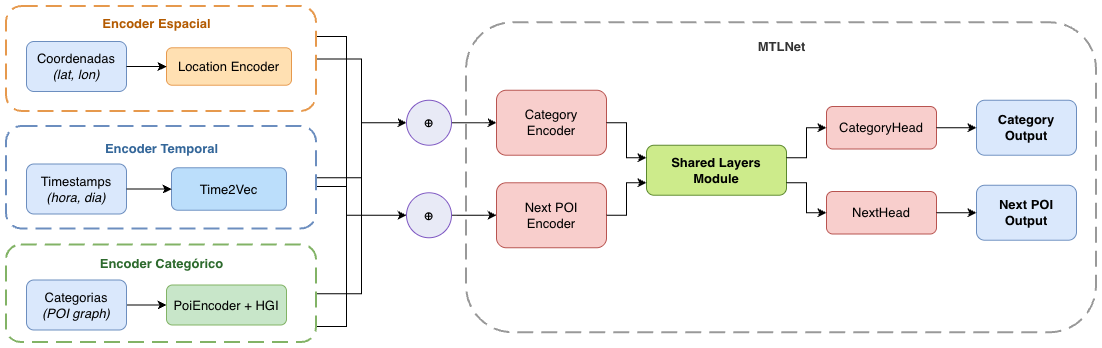
\includegraphics[width=1\textwidth]{imagens/arquitetura_modelo.png}}
    \caption{Arquitetura baseada no MTLNet \cite{silva2025mtlnet}. Os \textit{encoders} espacial, temporal e categórico são treinados de forma desacoplada e geram seus respectivos \textit{embeddings}, que são integrados como entrada do modelo e processados pelas camadas compartilhadas do modelo multitarefa (\textit{Shared Layers Module}) e pelas camadas específicas de cada tarefa, produzindo as saídas \textit{Category Output} e \textit{Next POI Output}.}
    \label{fig:arquitetura_arch}
\end{figure*}

O MTLNet \cite{silva2025mtlnet} é uma rede multitarefa construída sobre compartilhamento rígido de parâmetros (\textit{hard parameter sharing}) \cite{caruana1997multitask}, que processa simultaneamente as tarefas de classificação de categoria de POI e predição do próximo POI. A arquitetura utiliza \textit{encoders} específicos por tarefa implementados como MLPs com LayerNorm e Dropout, que projetam os \textit{embeddings} de entrada em um espaço latente compartilhado de dimensão $d_{\mathrm{shared}} = 256$. Em seguida, é aplicada a modulação FiLM (\textit{Feature-wise Linear Modulation}) \cite{perez2018film}, condicionada por um \textit{embedding} de identificador de tarefa $\mathbf{e}_{t}$, que gera parâmetros de escala $\gamma_{t}$ e deslocamento $\beta_{t}$ para modular as representações codificadas:

\begin{equation}
\mathrm{FiLM}(\mathbf{h}_{\mathrm{enc}}^{(t)} \,|\, \mathbf{e}_{t}) = \gamma_{t} \odot \mathbf{h}_{\mathrm{enc}}^{(t)} + \beta_{t}
\label{eq:film}
\end{equation}

As representações moduladas são processadas por quatro blocos residuais compartilhados com LayerNorm, LeakyReLU e Dropout, permitindo ao modelo aprender uma representação comum para ambas as tarefas \cite{baxter2000model}.

Na saída, cada tarefa possui uma \textit{head} especializada. O módulo de classificação de categoria utiliza um conjunto de três MLPs paralelas com profundidades variadas (2, 3 e 4 camadas), cujas saídas são concatenadas e projetadas para as 7 classes de POI. A \textit{head} de próximo POI emprega um \textit{Transformer encoder} com 8 \textit{heads} de atenção e 4 camadas, máscara causal para processamento autoregressivo, e \textit{pooling} ponderado por pesos de atenção aprendidos sobre os \textit{timesteps} da sequência de entrada. %(janela de tamanho $L_h = 9$).

O treinamento multitarefa utiliza o regularizador Nash-MTL \cite{nash}, que formula o balanceamento dos gradientes como um jogo cooperativo de barganha de Nash entre $K$ tarefas. Dados os gradientes de cada tarefa, o Nash-MTL busca a direção de atualização que maximiza o produto das utilidades de todas as tarefas, o que garante que a atualização seja benéfica para todas as tarefas simultaneamente, evitando a dominância de uma tarefa sobre a outra.


% \begin{equation}
% \Delta\boldsymbol{\theta}^{*} = \arg\max_{\Delta\boldsymbol{\theta} \in \mathcal{B}_\varepsilon}
% \sum_{k=1}^{K} \log\!\left(\mathbf{g}_k^{\top} \Delta\boldsymbol{\theta}\right)
% \quad\text{s.t. } \mathbf{g}_k^{\top} \Delta\boldsymbol{\theta} > 0,\;\forall k
% \label{eq:nash}
% \end{equation}

\subsection{Baseline: MTLNet com DGI}

O modelo \textit{baseline} corresponde ao MTLNet original proposto em \cite{silva2025mtlnet}, cuja arquitetura interna é mantida inalterada neste trabalho. Nesse modelo, cada POI é representado por um único \textit{embedding} monolítico $\mathbf{E}_{DGI} \in \mathbb{R}^{64}$, obtido via \textit{Deep Graph Infomax} (DGI) \cite{velickovic2019deep} sobre um grafo espacial construído por Triangulação de Delaunay e atributos categóricos dos nós, conforme descrito detalhadamente em \cite{silva2025mtlnet}. Assim, o DGI codifica conjuntamente relações espaciais e categóricas em um único vetor, sem incorporar componentes temporais explícitas. Em contraste, a abordagem proposta substitui essa representação monolítica pela concatenação de três \textit{encoders} especializados, totalizando 192 dimensões de entrada.


\subsection{Preparação dos Dados}

Para a tarefa de \textit{classificação de categoria de POI}, cada POI é representado pelo \textit{embedding} resultante da concatenação dos três componentes, $\mathbf{E}_{cat} = [\mathbf{E}_{HGI} \| \mathbf{E}_{loc} \| \mathbf{E}_{time}] \in \mathbb{R}^{192}$, formando pares $(\mathbf{E}_{cat}, c)$ onde $c$ é a categoria real do POI. No caso do \textit{baseline}, é utilizado diretamente $\mathbf{E}_{DGI} \in \mathbb{R}^{64}$.

Para a tarefa de \textit{predição do próximo POI}, os \textit{check-ins} são ordenados cronologicamente por usuário, e usuários com menos de cinco visitas são descartados. São extraídas janelas não sobrepostas de tamanho $L_h = 9$: os \textit{check-ins} $(p_1, \dots, p_9)$ formam o contexto, e $p_{\text{target}}$ é o próximo POI cuja categoria deve ser predita. Cada \textit{check-in} da janela é representado pelo \textit{embedding} correspondente, resultando em uma entrada de $9 \times 192 = 1728$ dimensões para o ST-MTLNet e $9 \times 64 = 576$ dimensões para o \textit{baseline}. Sequências mais curtas são preenchidas com \textit{padding} de vetores nulos.

\subsection{Encoder Espacial}

O modelo original MTLNet codifica informações espaciais de forma implícita por meio da topologia do grafo de Delaunay, sem utilizar diretamente as coordenadas geográficas como sinal de entrada. No entanto, como discutido na Seção~\ref{sec:related_works}, codificadores espaciais contínuos têm demonstrado eficácia em diversas tarefas geoespaciais \cite{wu2024torchspatial}, embora sua aplicação em modelos multitarefa de POIs permaneça pouco explorada. Este trabalho seleciona dois \textit{encoders} que representam paradigmas distintos de codificação espacial: o SIREN \cite{rußwurm2024geographiclocationencodingspherical}, que modela funções contínuas por ativações senoidais com frequências controláveis, e o Sphere2Vec-M \cite{mai2023sphere2vecgeneralpurposelocationrepresentation}, que opera diretamente em coordenadas esféricas preservando propriedades de distância geodésica. Essa diversidade permite avaliar como diferentes pressupostos geométricos e arquiteturais impactam o desempenho em tarefas de POI.

Todos os \textit{encoders} produzem $\mathbf{E}_{loc} \in \mathbb{R}^{64}$ e são 
treinados com a mesma função de perda contrastiva binária baseada na distância geográfica entre pares de coordenadas:
\begin{equation}
\mathcal{L}_{\text{loc}}(i,j)
=
- \left[
y_{ij}\,\log \sigma\!\left(\frac{\text{sim}(z_i,z_j)}{\tau}\right)
+
(1-y_{ij})
\log \left(1 - \sigma\!\left(\frac{\text{sim}(z_i,z_j)}{\tau}\right)\right)
\right]
\end{equation}

na qual $\sigma$ denota a função sigmoide, $\text{sim}(\cdot,\cdot)$ é a similaridade de cosseno, e $y_{ij} \in \{0,1\}$ indica se o par é positivo ($\Delta d_{ij} \leq 10$ km) ou negativo ($\Delta d_{ij} \geq 70$ km), com temperatura $\tau = 0{,}15$. A utilização da mesma função de perda para os dois \textit{encoders} espaciais permite uma comparação controlada, isolando o efeito da arquitetura de codificação.

% \subsubsection{Space2Vec-grid}

% O Space2Vec-grid proposto por Mai et al. \cite{mai2020multiscalerepresentationlearningspatial} realiza a modelagem espacial a partir das coordenadas contínuas de latitude e longitude dos \textit{check-ins} e pode ser definido em duas camadas principais:

% \begin{description}
%     \item[\textbf{Codificador Posicional Senoidal (\textit{Position Encoder}):}]
%     As coordenadas ($\lambda, \phi$) dos \textit{check-ins} são transformadas em um vetor de alta dimensão por meio de funções senoidais e cossenos com frequências logaritmicamente espaçadas.

%     \item[\textbf{Rede Neural \textit{Feed-Forward} (FFN):}]
%     O vetor de codificação posicional é processado por uma FFN de múltiplas camadas com \textit{skip connection} e LayerNorm, que projeta a representação no \textit{embedding} final $\mathbf{E}_{loc} \in \mathbb{R}^{64}$.
% \end{description}

\subsubsection{SIREN}

O modelo SIREN (\textit{Sinusoidal Representation Networks}) \cite{rußwurm2024geographiclocationencodingspherical} modela uma função contínua $f_\theta : \mathbb{R}^2 \rightarrow \mathbb{R}^{64}$ que mapeia diretamente coordenadas geográficas normalizadas em um \textit{embedding} vetorial. Cada camada da rede utiliza ativações senoidais com frequências controláveis, permitindo representar sinais de alta frequência em dados espaciais. A saída é o \textit{embedding} $\mathbf{E}_{loc} \in \mathbb{R}^{64}$.

\subsubsection{Sphere2Vec-M}

O Sphere2Vec-M \cite{mai2023sphere2vecgeneralpurposelocationrepresentation} é um codificador multi-escala formulado para operar diretamente em coordenadas esféricas ($\lambda$, $\phi$), gerando representações que preservem propriedades de distância na superfície da esfera. É utilizada a variante \textit{sphereM}, na qual são empregadas $S=16$ escalas multi-resolução com fatores geometricamente espaçados entre 10 km e 10.000 km. Termos de interação entre $\lambda$ e $\phi$ são construídos mantendo uma das componentes no maior nível de escala, permitindo controlar a resolução angular de latitude e longitude de forma independente. O vetor resultante é projetado por uma MLP para produzir $\mathbf{E}_{loc} \in \mathbb{R}^{64}$.

\subsection{Encoder Temporal}

Padrões de mobilidade humana apresentam regularidades cíclicas, como horários de refeição e deslocamentos semanais, que carregam informações discriminativas sobre a natureza funcional dos POIs visitados \cite{sun2020go}. No entanto, o modelo original MTLNet não incorpora representações temporais explícitas para capturar essas informações. 

Para preencher essa lacuna, é utilizado o Time2Vec \cite{kazemi2019time2vec}, uma representação temporal genérica e desacoplada capaz de capturar padrões periódicos e não periódicos sem necessidade de engenharia manual de \textit{features}. A arquitetura combina termos lineares e periódicos para mapear os valores temporais de cada \textit{check-in} (hora do dia e dia da semana, de forma acoplada) em um vetor de \textit{embedding}. Para um \textit{embedding} de dimensão $D$, a função é definida como:

\begin{equation}
\mathbf{f}(\tau)[i] = \begin{cases} \omega_0 \tau + \phi_0 & \text{se } i=0 \\ \sin(\omega_i \tau + \phi_i) & \text{se } 1 \leq i \leq D-1 \end{cases}
\label{eq:time2vec}
\end{equation}

na qual $\omega_i$ e $\phi_i$ são parâmetros treináveis (pesos e \textit{bias}) que capturam a periodicidade dos padrões temporais de visitação. O termo linear ($i=0$) captura tendências temporais globais, enquanto os termos senoidais modelam padrões cíclicos em diferentes frequências.

O modelo é treinado usando os valores temporais discretos (hora do dia e dia da semana) de forma acoplada para cada \textit{check-in}, com a mesma formulação contrastiva binária empregada no encoder espacial, sendo denominada $\mathcal{L}_{tempo}$. A saída final é o \textit{embedding} $\mathbf{E}_{time} \in \mathbb{R}^{64}$, que representa o \textit{timestamp} de cada \textit{check-in}.

\subsection{Encoder Categórico}

O DGI utilizado no modelo original codifica informações categóricas por meio de uma matriz \textit{one-hot} de 7 classes processada pela estrutura do grafo, sem capturar explicitamente relações hierárquicas ou regionais entre categorias de POIs. Para enriquecer essa dimensão, a geração de \textit{embeddings} categóricos é realizada em duas fases complementares. O POI Encoder aprende representações vetoriais que capturam coocorrências entre categorias a partir de caminhadas aleatórias no grafo espacial, e o modelo HGI \cite{huang2023learning} incorpora informações hierárquicas em múltiplos níveis (POI, região e cidade), produzindo representações que refletem tanto o contexto local quanto o regional.

\subsubsection{POI Encoder}

O POI Encoder é treinado de forma independente para gerar o \textit{embedding} de categoria $\mathbf{E}_{\text{POI\_categoria}} \in \mathbb{R}^{64}$. Os POIs são organizados em um grafo espacial construído por Triangulação de Delaunay sobre as coordenadas geográficas, com arestas ponderadas por decaimento logarítmico da distância Haversine e penalização para conexões entre condados (GEOIDs) distintos.

Sobre esse grafo são executadas caminhadas aleatórias (\textit{random walks}) seguindo a metodologia do Node2Vec \cite{grover2016node2vec}. Cada caminhada é convertida em uma sequência de categorias secundárias (\textit{fclass}), resultando em coocorrências locais e globais entre categorias. O modelo aprende os \textit{embeddings} utilizando a estratégia \textit{skip-gram} com \textit{negative sampling} \cite{church2017word2vec}:

\[
\mathcal{L}_{\text{SGNS}}(i,j)
=
-\log \sigma\!\left(\mathbf{e}_j^\top \mathbf{e}_i\right)
-
\sum_{k=1}^{K}
\log \sigma\!\left(-\mathbf{e}_{n_k}^\top \mathbf{e}_i\right),
\]

na qual $\mathbf{e}_i$ é o \textit{embedding} da classe alvo, $\mathbf{e}_j$ o \textit{embedding} positivo de contexto, e $\mathbf{e}_{n_k}$ representam as amostras negativas. A implementação incorpora um termo de regularização hierárquica \cite{belkin2003laplacian} entre categoria e \textit{fclass}: $\mathcal{L}_{\text{hier}} = \sum_{(c,s) \in \mathcal{H}} \left\| \mathbf{e}_s - \mathbf{e}_c \right\|_2^2$, na qual $\mathcal{H}$ contém os pares (categoria, \textit{fclass}). A perda total é $\mathcal{L} = \mathcal{L}_{\text{SGNS}} + \lambda_{\text{hier}} \, \mathcal{L}_{\text{hier}}$. Ao final, o \textit{embedding} resultante é gerado por categoria e remapeado para cada POI.

\subsubsection{Hierarchical Graph Infomax (HGI)}

Após a geração dos \textit{embeddings} $\mathbf{E}_{\text{POI\_categoria}}$, eles são utilizados como entrada para o modelo Hierarchical Graph Infomax (HGI) \cite{huang2023learning}, que enriquece a representação incorporando informações geográficas regionais. O modelo otimiza a informação mútua em dois níveis hierárquicos (POI-região e região-cidade):

\[
\mathcal{L}
=
\alpha\,\mathcal{L}_{\text{POI--região}}
+
(1-\alpha)\,\mathcal{L}_{\text{região--cidade}},
\]

na qual $\alpha = 0{,}5$ controla o equilíbrio entre os níveis hierárquicos. Ambas as perdas utilizam amostragem negativa estrutural para reforçar a separabilidade entre regiões e entre POIs. A saída são os \textit{embeddings} enriquecidos $\mathbf{E}_{\text{HGI}} \in \mathbb{R}^{64}$, que capturam relações categóricas tanto locais quanto regionais.



\subsection{Integração dos Embeddings}

Os três componentes de representação são treinados de forma independente e concatenados para formar a entrada de ambas as tarefas do MTLNet:

\begin{equation}
\mathbf{E}_{input} = [\mathbf{E}_{HGI} \| \mathbf{E}_{loc} \| \mathbf{E}_{time}] \in \mathbb{R}^{192}
\label{eq:concat}
\end{equation}

A escolha da concatenação como estratégia de integração preserva a informação individual de cada componente sem impor interações prematuras entre as representações, delegando ao MTLNet a tarefa de aprender como combinar essas dimensões por meio de suas camadas compartilhadas e da modulação FiLM. A dimensionalidade de entrada do ST-MTLNet ($\mathbb{R}^{192}$) é superior à do \textit{baseline} ($\mathbb{R}^{64}$), uma consequência natural da decomposição em três componentes. No entanto, a arquitetura do MTLNet projeta qualquer entrada para o mesmo espaço latente compartilhado de dimensão $d_{\mathrm{shared}} = 256$ por meio dos \textit{encoders} específicos por tarefa, de modo que a capacidade das camadas compartilhadas e das cabeças de tarefa permanece inalterada.

São avaliadas duas variantes do modelo proposto, denominadas ST-MTLNet (\textit{Spatial-Temporal MTLNet}), cada uma utilizando um \textit{encoder} espacial diferente. O \textit{baseline} MTLNet \cite{silva2025mtlnet} utiliza somente o \textit{embedding} monolítico $\mathbf{E}_{DGI} \in \mathbb{R}^{64}$ como entrada para ambas as tarefas. As variantes propostas substituem essa representação pela concatenação dos \textit{embeddings} desacoplados, mantendo fixos os \textit{encoders} temporal (Time2Vec) e categórico (HGI) e variando o \textit{encoder} espacial entre SIREN e Sphere2Vec-M.

Todos os modelos compartilham os mesmos hiperparâmetros da arquitetura MTLNet, diferindo apenas nos \textit{embeddings} de entrada. Essa configuração permite isolar o efeito da estratégia de representação sobre o desempenho, avaliando tanto o ganho da abordagem modular em relação ao \textit{baseline} monolítico quanto o impacto da escolha do \textit{encoder} espacial.

\section{Resultados} \label{sec:results}
\subsection{Configuração Experimental}

O desempenho dos modelos é avaliado por meio do F1-Score médio por categoria, reportado como média e desvio padrão em 5 \textit{folds} com divisão estratificada, utilizando 80\% dos dados para treino e 20\% para validação, preservando a proporção entre categorias.

\begin{table}[htbp]
\centering
\caption{Total de \textit{check-ins}, POIs, e usuários de Flórida, Califórnia e Texas.}
\label{tab:dataset}
\begin{tabular}{lccc}
\hline
Estados & \textit{Check-ins} & Pontos de Interesse & Usuários \\
\hline
Florida & 990.518 & 65.009 & 20.301 \\
California & 2.535.573 & 148.314 & 36.106 \\
Texas & 3.355.419 & 135.570 & 37.522 \\
\hline
\end{tabular}
\end{table}

Os experimentos foram conduzidos com o \textit{dataset} Gowalla \cite{10.1145/2661829.2662002} nos estados da Flórida, Califórnia e Texas, cujas estatísticas são apresentadas na Tabela \ref{tab:dataset}. A escolha desses estados se deve ao elevado volume de \textit{check-ins} e à presença de padrões urbanos e distribuições espaciais distintas, o que permite avaliar o comportamento dos modelos em cenários com diferentes níveis de densidade e dispersão geográfica.

\begin{figure}[htbp]
    \centering
    
\includegraphics[width=\textwidth]{imagens/subáreas/distribuicao_estados.png}
    \caption{Distribuição espacial de POIs das categorias Food (vermelho) e Shopping (laranja) na sub-região mais densa de Flórida, Califórnia e Texas. As sub-regiões foram selecionadas por densidade em \textit{grid}, com cerca de 100 POIs por região.}
    \label{fig:distribuicao_espacial}
\end{figure}

\begin{table}[ht]
\centering
\caption{\textnormal{F1-Score Médio (\%) por modelo e estado para a tarefa de Classificação de Categoria de POI.}}
\label{table:poi_category}
\vspace{0.3cm}
\resizebox{\textwidth}{!}{%
\begin{tabular}{cl|c|c|c|}
\hline
\multicolumn{2}{c|}{} & \textbf{MTLNet} & \textbf{ST-MTLNet$_{SIREN}$} & \textbf{ST-MTLNet$_{Sphere2Vec-M}$} \\ \hline
\multirow{7}{*}{\textbf{Florida}} & Community & 51,86 ± 0,73 & \textbf{70,00 ± 0,81} & 69,84 ± 0,98 \\
 & Entertainment & 41,24 ± 1,83 & \textbf{64,45 ± 1,82} & 63,92 ± 1,61 \\
 & Food & 55,47 ± 1,55 & 72,92 ± 0,59 & \textbf{73,22 ± 0,66} \\
 & Nightlife & 32,59 ± 1,96 & \textbf{62,60 ± 1,96} & 62,44 ± 2,00 \\
 & Outdoors & 47,71 ± 1,60 & 65,64 ± 1,73 & \textbf{66,35 ± 1,51} \\
 & Shopping & 62,96 ± 0,62 & \textbf{77,48 ± 0,36} & 77,47 ± 0,72 \\
 & Travel & 45,49 ± 1,20 & \textbf{64,89 ± 1,20} & 64,77 ± 1,54 \\
\hline
\multirow{7}{*}{\textbf{California}} & Community & 53,22 ± 0,37 & \textbf{70,21 ± 0,17} & 70,08 ± 0,44 \\
 & Entertainment & 40,89 ± 1,32 & \textbf{63,60 ± 0,83} & 63,21 ± 0,76 \\
 & Food & 60,68 ± 0,69 & \textbf{75,78 ± 0,39} & 75,74 ± 0,19 \\
 & Nightlife & 26,81 ± 1,71 & 60,59 ± 1,35 & \textbf{60,78 ± 1,63} \\
 & Outdoors & 51,59 ± 1,15 & \textbf{67,94 ± 1,52} & 67,37 ± 1,95 \\
 & Shopping & 60,43 ± 1,01 & 76,84 ± 0,29 & \textbf{77,00 ± 0,33} \\
 & Travel & 38,88 ± 1,32 & \textbf{63,59 ± 1,45} & 63,25 ± 0,99 \\
\hline
\multirow{7}{*}{\textbf{Texas}} & Community & 57,37 ± 0,69 & 73,45 ± 0,34 & \textbf{76,20 ± 0,46} \\
 & Entertainment & 46,69 ± 0,46 & 64,09 ± 1,24 & \textbf{67,73 ± 1,43} \\
 & Food & 54,31 ± 0,42 & 69,80 ± 0,80 & \textbf{73,10 ± 0,17} \\
 & Nightlife & 34,44 ± 1,21 & 60,62 ± 1,32 & \textbf{64,57 ± 1,03} \\
 & Outdoors & 45,99 ± 1,70 & 64,21 ± 0,42 & \textbf{68,72 ± 0,70} \\
 & Shopping & 62,70 ± 0,29 & 76,40 ± 0,44 & \textbf{79,67 ± 0,14} \\
 & Travel & 39,37 ± 1,29 & 57,53 ± 1,08 & \textbf{64,73 ± 0,72} \\
\hline
\end{tabular}}
\end{table}

\subsection{Classificação de Categoria de POI}

Os resultados da tarefa de classificação de categoria de POI são apresentados na Tabela \ref{table:poi_category}. Nos três estados avaliados, as duas variantes do ST-MTLNet superam o MTLNet original em todas as 21 combinações de categoria e estado, evidenciando que a substituição do \textit{embedding} monolítico do DGI por representações desacopladas enriquece de forma consistente a caracterização dos POIs. Os ganhos são particularmente expressivos em categorias como \textit{Nightlife} e \textit{Travel}. Em \textit{Nightlife}, por exemplo, o ST-MTLNet com Sphere2Vec-M atinge 62,44 $\pm$ 2,00 na Flórida, 60,78 $\pm$ 1,63 na Califórnia e 64,57 $\pm$ 1,03 no Texas, sempre muito acima do \textit{baseline}. Em \textit{Travel}, os melhores resultados chegam a 64,89 $\pm$ 1,20 na Flórida com SIREN, 63,59 $\pm$ 1,45 na Califórnia com SIREN e 64,73 $\pm$ 0,72 no Texas com Sphere2Vec-M.

As melhorias observadas em \textit{Food} e \textit{Shopping} reforçam que a localização geográfica carrega sinais discriminativos relevantes para a categoria semântica do POI. A Figura \ref{fig:distribuicao_espacial} mostra que essas categorias tendem a formar aglomerados densos nas sub-regiões analisadas, favorecendo a captura de padrões espaciais pelos \textit{encoders} contínuos. Embora as duas variantes propostas apresentem desempenho próximo, observa-se um comportamento complementar: o SIREN obtém mais resultados de destaque na Flórida e na Califórnia, enquanto o Sphere2Vec-M se destaca com maior frequência no Texas. Em conjunto, esses resultados mostram que a abordagem modular supera de forma consistente o paradigma monolítico do DGI nessa tarefa.

\begin{table}[ht]
\centering
\caption{\textnormal{F1-Score Médio (\%) por modelo e estado para a tarefa de Predição de Próximo POI.}}
\label{table:next}
\vspace{0.3cm}
\resizebox{\textwidth}{!}{%
\begin{tabular}{cl|c|c|c|}
\hline
\multicolumn{2}{c|}{} & \textbf{MTLNet} & \textbf{ST-MTLNet$_{SIREN}$} & \textbf{ST-MTLNet$_{Sphere2Vec-M}$} \\ \hline
\multirow{7}{*}{\textbf{Florida}} & Community & 34,33 ± 1,33 & \textbf{38,31 ± 0,90} & 37,98 ± 1,22 \\
 & Entertainment & 25,34 ± 1,07 & \textbf{31,38 ± 1,72} & 31,24 ± 2,41 \\
 & Food & 27,12 ± 2,79 & \textbf{41,91 ± 1,93} & 41,65 ± 3,15 \\
 & Nightlife & 21,33 ± 1,61 & 23,32 ± 2,74 & \textbf{23,98 ± 1,94} \\
 & Outdoors & \textbf{21,61 ± 0,99} & 21,29 ± 1,59 & 21,59 ± 1,91 \\
 & Shopping & 39,62 ± 3,40 & 44,00 ± 2,04 & \textbf{44,66 ± 2,38} \\
 & Travel & \textbf{64,47 ± 1,02} & 45,00 ± 1,10 & 44,93 ± 1,11 \\
\hline
\multirow{7}{*}{\textbf{California}} & Community & 32,14 ± 0,89 & \textbf{37,86 ± 0,20} & 37,80 ± 1,11 \\
 & Entertainment & \textbf{19,38 ± 0,94} & 17,28 ± 1,73 & 17,01 ± 1,39 \\
 & Food & 29,26 ± 1,67 & 50,42 ± 1,15 & \textbf{51,28 ± 0,57} \\
 & Nightlife & \textbf{18,24 ± 0,53} & 16,34 ± 1,95 & 15,10 ± 2,70 \\
 & Outdoors & \textbf{25,01 ± 0,81} & 24,84 ± 1,70 & 24,07 ± 2,46 \\
 & Shopping & 38,41 ± 2,64 & \textbf{39,04 ± 1,72} & 37,82 ± 1,31 \\
 & Travel & \textbf{46,05 ± 0,84} & 36,94 ± 1,70 & 37,82 ± 1,04 \\
\hline
\multirow{7}{*}{\textbf{Texas}} & Community & 34,22 ± 0,43 & 35,99 ± 0,93 & \textbf{36,97 ± 0,81} \\
 & Entertainment & 25,56 ± 1,56 & \textbf{28,30 ± 1,37} & 27,59 ± 1,64 \\
 & Food & 29,56 ± 4,10 & 47,48 ± 2,42 & \textbf{48,67 ± 0,66} \\
 & Nightlife & 25,46 ± 1,13 & 26,06 ± 1,36 & \textbf{26,14 ± 2,66} \\
 & Outdoors & 23,02 ± 1,03 & \textbf{24,62 ± 0,46} & 23,04 ± 1,44 \\
 & Shopping & 38,79 ± 4,12 & \textbf{45,40 ± 1,30} & 43,18 ± 2,19 \\
 & Travel & 29,71 ± 1,32 & \textbf{34,26 ± 0,90} & 33,05 ± 1,51 \\
\hline
\end{tabular}}
\end{table}

\subsection{Predição do Próximo POI}

Os resultados da tarefa de predição do próximo POI são apresentados na Tabela \ref{table:next}. Diferentemente do que ocorre na classificação, essa tarefa apresenta um cenário mais heterogêneo, mas ainda favorável às variantes propostas: os modelos espaço-temporais superam o MTLNet original em 16 das 21 combinações avaliadas. Os ganhos mais expressivos ocorrem em \textit{Food}, categoria em que ambas as variantes superam o \textit{baseline} nos três estados. O melhor resultado é obtido pelo Sphere2Vec-M no Texas, com 48,67 $\pm$ 0,66, enquanto na Califórnia o mesmo modelo alcança 51,28 $\pm$ 0,57, superando com ampla margem o DGI. Melhorias consistentes também aparecem em \textit{Shopping} e \textit{Community}, sugerindo que a combinação entre informação espacial contínua e contexto temporal favorece a modelagem de transições recorrentes entre categorias.

O padrão de co-localização mostrado na Figura \ref{fig:distribuicao_espacial} ajuda a interpretar esse comportamento, pois a presença de agrupamentos densos de categorias como \textit{Food} e \textit{Shopping} favorece transições locais frequentes ao longo da trajetória do usuário. Ainda assim, o \textit{baseline} mantém vantagem em alguns casos, especialmente em \textit{Travel} na Flórida e na Califórnia, além de categorias específicas na Califórnia, como \textit{Entertainment}, \textit{Nightlife} e \textit{Outdoors}. Esses resultados sugerem que deslocamentos de longa distância e relações topológicas entre regiões ainda são melhor representados pelo DGI, cujo grafo espacial captura conexões estruturais que os \textit{encoders} baseados em coordenadas não modelam diretamente. Mesmo com essa limitação, o desempenho geral indica que as representações propostas são mais eficazes na maioria dos cenários de predição sequencial.


\section{Conclusão e Trabalhos Futuros} \label{sec:conclusion}
Este trabalho investigou se a substituição do \textit{embedding} monolítico do DGI por representações desacopladas e especializadas poderia produzir uma base mais adequada para as tarefas de classificação de categoria de POI e predição do próximo POI. Os resultados obtidos nos três estados avaliados indicam que sim. Ao incorporar um \textit{encoder} espacial contínuo, um \textit{encoder} temporal (Time2Vec) e um \textit{encoder} categórico hierárquico (HGI), o ST-MTLNet supera de forma consistente o \textit{baseline} baseado apenas em DGI.

Na tarefa de classificação de categoria de POI, as variantes propostas superam o MTLNet em todas as 21 combinações de categoria e estado, com ganhos médios de 20 a 24 pontos percentuais. Na tarefa de predição do próximo POI, o desempenho também é majoritariamente favorável ao ST-MTLNet, que vence em 16 das 21 combinações avaliadas, com destaque para categorias como \textit{Food}. Em conjunto, esses resultados mostram que a decomposição da representação em componentes espaciais, temporais e categóricos permite capturar padrões que o DGI, por si só, não modela de forma suficiente.

A comparação entre SIREN e Sphere2Vec-M também mostra que não há um único \textit{encoder} espacial universalmente superior. O SIREN apresenta melhor desempenho com maior frequência na Flórida e na Califórnia, enquanto o Sphere2Vec-M se destaca no Texas, sugerindo que a adequação do \textit{encoder} depende da distribuição geográfica dos POIs em cada território. Assim, o principal ganho do trabalho não está apenas na escolha de uma arquitetura espacial específica, mas na própria adoção de representações desacopladas como alternativa ao paradigma monolítico do DGI.

Uma limitação relevante permanece na categoria \textit{Travel} da tarefa de predição do próximo POI, na qual o MTLNet original ainda obtém os melhores resultados em parte dos cenários. Isso sugere que deslocamentos de longa distância e relações topológicas entre regiões ainda são melhor capturados pela estrutura de grafo utilizada pelo DGI. Além disso, como os três componentes propostos são utilizados em conjunto, este trabalho não isola a contribuição individual de cada \textit{encoder}, o que restringe uma análise mais detalhada sobre o peso relativo de cada fonte de informação.

Como trabalhos futuros, destacam-se a investigação de arquiteturas multitarefa mais flexíveis, a exploração de estratégias de fusão mais sofisticadas entre os \textit{encoders} e a combinação entre representações baseadas em grafo e codificações contínuas de coordenadas. Essas direções podem ampliar os ganhos observados e ajudar a reduzir as limitações ainda presentes em categorias como \textit{Travel}.

\bibliographystyle{sbc}
\bibliography{references}

% \bibliography{sbc-template}

\end{document}